\addcontentsline{toc}{chapter}{Приложение}
\hypertarget{apA}{}
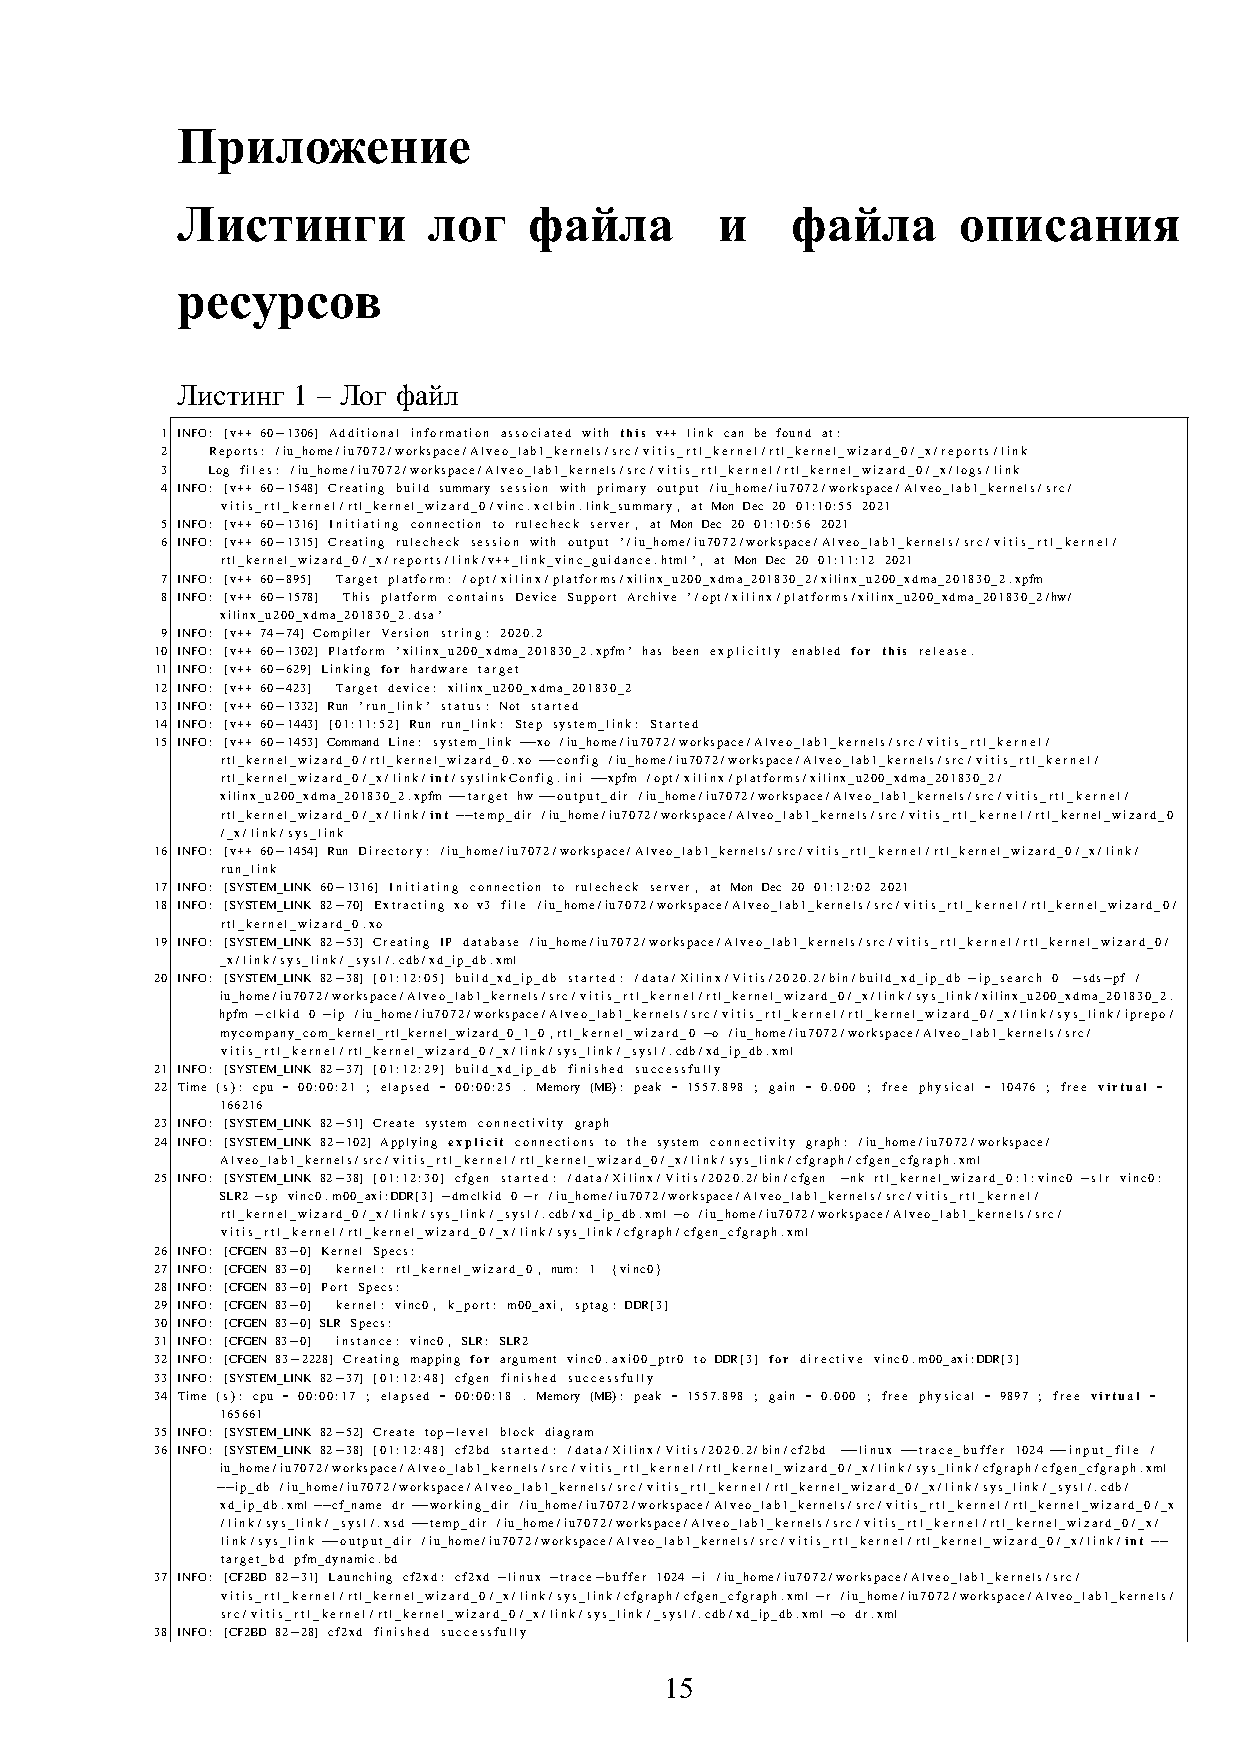
\includepdf[pages=-]{08-A.pdf}

% \chapter*{\hypertarget{apA}{}Приложение\\Листинги лог~файла~~и~~файла описания
%                              ресурсов}
% 
% \begin{center}
%     \captionsetup{justification=raggedright,singlelinecheck=off}
%     \begin{lstlisting}[label=lst:vlog,caption=Лог файл]
% INFO: [v++ 60-1306] Additional information associated with this v++ link can be found at:
% 	Reports: /iu_home/iu7072/workspace/Alveo_lab1_kernels/src/vitis_rtl_kernel/rtl_kernel_wizard_0/_x/reports/link
% 	Log files: /iu_home/iu7072/workspace/Alveo_lab1_kernels/src/vitis_rtl_kernel/rtl_kernel_wizard_0/_x/logs/link
% INFO: [v++ 60-1548] Creating build summary session with primary output /iu_home/iu7072/workspace/Alveo_lab1_kernels/src/vitis_rtl_kernel/rtl_kernel_wizard_0/vinc.xclbin.link_summary, at Mon Dec 20 01:10:55 2021
% INFO: [v++ 60-1316] Initiating connection to rulecheck server, at Mon Dec 20 01:10:56 2021
% INFO: [v++ 60-1315] Creating rulecheck session with output '/iu_home/iu7072/workspace/Alveo_lab1_kernels/src/vitis_rtl_kernel/rtl_kernel_wizard_0/_x/reports/link/v++_link_vinc_guidance.html', at Mon Dec 20 01:11:12 2021
% INFO: [v++ 60-895]   Target platform: /opt/xilinx/platforms/xilinx_u200_xdma_201830_2/xilinx_u200_xdma_201830_2.xpfm
% INFO: [v++ 60-1578]   This platform contains Device Support Archive '/opt/xilinx/platforms/xilinx_u200_xdma_201830_2/hw/xilinx_u200_xdma_201830_2.dsa'
% INFO: [v++ 74-74] Compiler Version string: 2020.2
% INFO: [v++ 60-1302] Platform 'xilinx_u200_xdma_201830_2.xpfm' has been explicitly enabled for this release.
% INFO: [v++ 60-629] Linking for hardware target
% INFO: [v++ 60-423]   Target device: xilinx_u200_xdma_201830_2
% INFO: [v++ 60-1332] Run 'run_link' status: Not started
% INFO: [v++ 60-1443] [01:11:52] Run run_link: Step system_link: Started
% INFO: [v++ 60-1453] Command Line: system_link --xo /iu_home/iu7072/workspace/Alveo_lab1_kernels/src/vitis_rtl_kernel/rtl_kernel_wizard_0/rtl_kernel_wizard_0.xo --config /iu_home/iu7072/workspace/Alveo_lab1_kernels/src/vitis_rtl_kernel/rtl_kernel_wizard_0/_x/link/int/syslinkConfig.ini --xpfm /opt/xilinx/platforms/xilinx_u200_xdma_201830_2/xilinx_u200_xdma_201830_2.xpfm --target hw --output_dir /iu_home/iu7072/workspace/Alveo_lab1_kernels/src/vitis_rtl_kernel/rtl_kernel_wizard_0/_x/link/int --temp_dir /iu_home/iu7072/workspace/Alveo_lab1_kernels/src/vitis_rtl_kernel/rtl_kernel_wizard_0/_x/link/sys_link
% INFO: [v++ 60-1454] Run Directory: /iu_home/iu7072/workspace/Alveo_lab1_kernels/src/vitis_rtl_kernel/rtl_kernel_wizard_0/_x/link/run_link
% INFO: [SYSTEM_LINK 60-1316] Initiating connection to rulecheck server, at Mon Dec 20 01:12:02 2021
% INFO: [SYSTEM_LINK 82-70] Extracting xo v3 file /iu_home/iu7072/workspace/Alveo_lab1_kernels/src/vitis_rtl_kernel/rtl_kernel_wizard_0/rtl_kernel_wizard_0.xo
% INFO: [SYSTEM_LINK 82-53] Creating IP database /iu_home/iu7072/workspace/Alveo_lab1_kernels/src/vitis_rtl_kernel/rtl_kernel_wizard_0/_x/link/sys_link/_sysl/.cdb/xd_ip_db.xml
% INFO: [SYSTEM_LINK 82-38] [01:12:05] build_xd_ip_db started: /data/Xilinx/Vitis/2020.2/bin/build_xd_ip_db -ip_search 0  -sds-pf /iu_home/iu7072/workspace/Alveo_lab1_kernels/src/vitis_rtl_kernel/rtl_kernel_wizard_0/_x/link/sys_link/xilinx_u200_xdma_201830_2.hpfm -clkid 0 -ip /iu_home/iu7072/workspace/Alveo_lab1_kernels/src/vitis_rtl_kernel/rtl_kernel_wizard_0/_x/link/sys_link/iprepo/mycompany_com_kernel_rtl_kernel_wizard_0_1_0,rtl_kernel_wizard_0 -o /iu_home/iu7072/workspace/Alveo_lab1_kernels/src/vitis_rtl_kernel/rtl_kernel_wizard_0/_x/link/sys_link/_sysl/.cdb/xd_ip_db.xml
% INFO: [SYSTEM_LINK 82-37] [01:12:29] build_xd_ip_db finished successfully
% Time (s): cpu = 00:00:21 ; elapsed = 00:00:25 . Memory (MB): peak = 1557.898 ; gain = 0.000 ; free physical = 10476 ; free virtual = 166216
% INFO: [SYSTEM_LINK 82-51] Create system connectivity graph
% INFO: [SYSTEM_LINK 82-102] Applying explicit connections to the system connectivity graph: /iu_home/iu7072/workspace/Alveo_lab1_kernels/src/vitis_rtl_kernel/rtl_kernel_wizard_0/_x/link/sys_link/cfgraph/cfgen_cfgraph.xml
% INFO: [SYSTEM_LINK 82-38] [01:12:30] cfgen started: /data/Xilinx/Vitis/2020.2/bin/cfgen  -nk rtl_kernel_wizard_0:1:vinc0 -slr vinc0:SLR2 -sp vinc0.m00_axi:DDR[3] -dmclkid 0 -r /iu_home/iu7072/workspace/Alveo_lab1_kernels/src/vitis_rtl_kernel/rtl_kernel_wizard_0/_x/link/sys_link/_sysl/.cdb/xd_ip_db.xml -o /iu_home/iu7072/workspace/Alveo_lab1_kernels/src/vitis_rtl_kernel/rtl_kernel_wizard_0/_x/link/sys_link/cfgraph/cfgen_cfgraph.xml
% INFO: [CFGEN 83-0] Kernel Specs: 
% INFO: [CFGEN 83-0]   kernel: rtl_kernel_wizard_0, num: 1  {vinc0}
% INFO: [CFGEN 83-0] Port Specs: 
% INFO: [CFGEN 83-0]   kernel: vinc0, k_port: m00_axi, sptag: DDR[3]
% INFO: [CFGEN 83-0] SLR Specs: 
% INFO: [CFGEN 83-0]   instance: vinc0, SLR: SLR2
% INFO: [CFGEN 83-2228] Creating mapping for argument vinc0.axi00_ptr0 to DDR[3] for directive vinc0.m00_axi:DDR[3]
% INFO: [SYSTEM_LINK 82-37] [01:12:48] cfgen finished successfully
% Time (s): cpu = 00:00:17 ; elapsed = 00:00:18 . Memory (MB): peak = 1557.898 ; gain = 0.000 ; free physical = 9897 ; free virtual = 165661
% INFO: [SYSTEM_LINK 82-52] Create top-level block diagram
% INFO: [SYSTEM_LINK 82-38] [01:12:48] cf2bd started: /data/Xilinx/Vitis/2020.2/bin/cf2bd  --linux --trace_buffer 1024 --input_file /iu_home/iu7072/workspace/Alveo_lab1_kernels/src/vitis_rtl_kernel/rtl_kernel_wizard_0/_x/link/sys_link/cfgraph/cfgen_cfgraph.xml --ip_db /iu_home/iu7072/workspace/Alveo_lab1_kernels/src/vitis_rtl_kernel/rtl_kernel_wizard_0/_x/link/sys_link/_sysl/.cdb/xd_ip_db.xml --cf_name dr --working_dir /iu_home/iu7072/workspace/Alveo_lab1_kernels/src/vitis_rtl_kernel/rtl_kernel_wizard_0/_x/link/sys_link/_sysl/.xsd --temp_dir /iu_home/iu7072/workspace/Alveo_lab1_kernels/src/vitis_rtl_kernel/rtl_kernel_wizard_0/_x/link/sys_link --output_dir /iu_home/iu7072/workspace/Alveo_lab1_kernels/src/vitis_rtl_kernel/rtl_kernel_wizard_0/_x/link/int --target_bd pfm_dynamic.bd
% INFO: [CF2BD 82-31] Launching cf2xd: cf2xd -linux -trace-buffer 1024 -i /iu_home/iu7072/workspace/Alveo_lab1_kernels/src/vitis_rtl_kernel/rtl_kernel_wizard_0/_x/link/sys_link/cfgraph/cfgen_cfgraph.xml -r /iu_home/iu7072/workspace/Alveo_lab1_kernels/src/vitis_rtl_kernel/rtl_kernel_wizard_0/_x/link/sys_link/_sysl/.cdb/xd_ip_db.xml -o dr.xml
% INFO: [CF2BD 82-28] cf2xd finished successfully
% INFO: [CF2BD 82-31] Launching cf_xsd: cf_xsd -disable-address-gen -bd pfm_dynamic.bd -dn dr -dp /iu_home/iu7072/workspace/Alveo_lab1_kernels/src/vitis_rtl_kernel/rtl_kernel_wizard_0/_x/link/sys_link/_sysl/.xsd
% INFO: [CF2BD 82-28] cf_xsd finished successfully
% INFO: [SYSTEM_LINK 82-37] [01:13:00] cf2bd finished successfully
% Time (s): cpu = 00:00:08 ; elapsed = 00:00:12 . Memory (MB): peak = 1557.898 ; gain = 0.000 ; free physical = 11761 ; free virtual = 167528
% INFO: [v++ 60-1441] [01:13:00] Run run_link: Step system_link: Completed
% Time (s): cpu = 00:00:59 ; elapsed = 00:01:09 . Memory (MB): peak = 1585.129 ; gain = 0.000 ; free physical = 11777 ; free virtual = 167540
% INFO: [v++ 60-1443] [01:13:00] Run run_link: Step cf2sw: Started
% INFO: [v++ 60-1453] Command Line: cf2sw -sdsl /iu_home/iu7072/workspace/Alveo_lab1_kernels/src/vitis_rtl_kernel/rtl_kernel_wizard_0/_x/link/int/sdsl.dat -rtd /iu_home/iu7072/workspace/Alveo_lab1_kernels/src/vitis_rtl_kernel/rtl_kernel_wizard_0/_x/link/int/cf2sw.rtd -nofilter /iu_home/iu7072/workspace/Alveo_lab1_kernels/src/vitis_rtl_kernel/rtl_kernel_wizard_0/_x/link/int/cf2sw_full.rtd -xclbin /iu_home/iu7072/workspace/Alveo_lab1_kernels/src/vitis_rtl_kernel/rtl_kernel_wizard_0/_x/link/int/xclbin_orig.xml -o /iu_home/iu7072/workspace/Alveo_lab1_kernels/src/vitis_rtl_kernel/rtl_kernel_wizard_0/_x/link/int/xclbin_orig.1.xml
% INFO: [v++ 60-1454] Run Directory: /iu_home/iu7072/workspace/Alveo_lab1_kernels/src/vitis_rtl_kernel/rtl_kernel_wizard_0/_x/link/run_link
% INFO: [v++ 60-1441] [01:13:13] Run run_link: Step cf2sw: Completed
% Time (s): cpu = 00:00:10 ; elapsed = 00:00:13 . Memory (MB): peak = 1585.129 ; gain = 0.000 ; free physical = 9336 ; free virtual = 165089
% INFO: [v++ 60-1443] [01:13:13] Run run_link: Step rtd2_system_diagram: Started
% INFO: [v++ 60-1453] Command Line: rtd2SystemDiagram
% INFO: [v++ 60-1454] Run Directory: /iu_home/iu7072/workspace/Alveo_lab1_kernels/src/vitis_rtl_kernel/rtl_kernel_wizard_0/_x/link/run_link
% INFO: [v++ 60-1441] [01:13:20] Run run_link: Step rtd2_system_diagram: Completed
% Time (s): cpu = 00:00:00 ; elapsed = 00:00:08 . Memory (MB): peak = 1585.129 ; gain = 0.000 ; free physical = 8380 ; free virtual = 164133
% INFO: [v++ 60-1443] [01:13:20] Run run_link: Step vpl: Started
% INFO: [v++ 60-1453] Command Line: vpl -t hw -f xilinx_u200_xdma_201830_2 --remote_ip_cache /iu_home/iu7072/workspace/Alveo_lab1_kernels/src/vitis_rtl_kernel/rtl_kernel_wizard_0/.ipcache --output_dir /iu_home/iu7072/workspace/Alveo_lab1_kernels/src/vitis_rtl_kernel/rtl_kernel_wizard_0/_x/link/int --log_dir /iu_home/iu7072/workspace/Alveo_lab1_kernels/src/vitis_rtl_kernel/rtl_kernel_wizard_0/_x/logs/link --report_dir /iu_home/iu7072/workspace/Alveo_lab1_kernels/src/vitis_rtl_kernel/rtl_kernel_wizard_0/_x/reports/link --config /iu_home/iu7072/workspace/Alveo_lab1_kernels/src/vitis_rtl_kernel/rtl_kernel_wizard_0/_x/link/int/vplConfig.ini -k /iu_home/iu7072/workspace/Alveo_lab1_kernels/src/vitis_rtl_kernel/rtl_kernel_wizard_0/_x/link/int/kernel_info.dat --webtalk_flag Vitis --temp_dir /iu_home/iu7072/workspace/Alveo_lab1_kernels/src/vitis_rtl_kernel/rtl_kernel_wizard_0/_x/link --no-info --iprepo /iu_home/iu7072/workspace/Alveo_lab1_kernels/src/vitis_rtl_kernel/rtl_kernel_wizard_0/_x/link/int/xo/ip_repo/mycompany_com_kernel_rtl_kernel_wizard_0_1_0 --messageDb /iu_home/iu7072/workspace/Alveo_lab1_kernels/src/vitis_rtl_kernel/rtl_kernel_wizard_0/_x/link/run_link/vpl.pb /iu_home/iu7072/workspace/Alveo_lab1_kernels/src/vitis_rtl_kernel/rtl_kernel_wizard_0/_x/link/int/dr.bd.tcl
% INFO: [v++ 60-1454] Run Directory: /iu_home/iu7072/workspace/Alveo_lab1_kernels/src/vitis_rtl_kernel/rtl_kernel_wizard_0/_x/link/run_link
% 
% ****** vpl v2020.2 (64-bit)
%   **** SW Build (by xbuild) on 2020-11-18-05:13:29
%     ** Copyright 1986-2020 Xilinx, Inc. All Rights Reserved.
% 
% INFO: [VPL 60-839] Read in kernel information from file '/iu_home/iu7072/workspace/Alveo_lab1_kernels/src/vitis_rtl_kernel/rtl_kernel_wizard_0/_x/link/int/kernel_info.dat'.
% INFO: [VPL 74-74] Compiler Version string: 2020.2
% INFO: [VPL 60-423]   Target device: xilinx_u200_xdma_201830_2
% INFO: [VPL 60-1032] Extracting hardware platform to /iu_home/iu7072/workspace/Alveo_lab1_kernels/src/vitis_rtl_kernel/rtl_kernel_wizard_0/_x/link/vivado/vpl/.local/hw_platform
% WARNING: /data/Xilinx/Vitis/2020.2/tps/lnx64/jre9.0.4 does not exist.
% [01:18:24] Run vpl: Step create_project: Started
% Creating Vivado project.
% [01:18:51] Run vpl: Step create_project: Completed
% [01:18:51] Run vpl: Step create_bd: Started
% [01:20:31] Run vpl: Step create_bd: RUNNING...
% [01:22:10] Run vpl: Step create_bd: RUNNING...
% [01:23:53] Run vpl: Step create_bd: RUNNING...
% [01:25:50] Run vpl: Step create_bd: RUNNING...
% [01:27:22] Run vpl: Step create_bd: RUNNING...
% [01:28:07] Run vpl: Step create_bd: Completed
% [01:28:07] Run vpl: Step update_bd: Started
% [01:28:09] Run vpl: Step update_bd: Completed
% [01:28:09] Run vpl: Step generate_target: Started
% [01:29:53] Run vpl: Step generate_target: RUNNING...
% [01:31:44] Run vpl: Step generate_target: RUNNING...
% [01:33:22] Run vpl: Step generate_target: RUNNING...
% [01:35:13] Run vpl: Step generate_target: RUNNING...
% [01:37:04] Run vpl: Step generate_target: RUNNING...
% [01:39:11] Run vpl: Step generate_target: Completed
% [01:39:11] Run vpl: Step config_hw_runs: Started
% [01:39:12] Run vpl: Step generate_target: RUNNING...
% [01:41:00] Run vpl: Step config_hw_runs: Completed
% [01:41:00] Run vpl: Step synth: Started
% [01:44:18] Block-level synthesis in progress, 0 of 66 jobs complete, 8 jobs running.
% [01:45:31] Block-level synthesis in progress, 0 of 66 jobs complete, 8 jobs running.
% [01:46:48] Block-level synthesis in progress, 0 of 66 jobs complete, 8 jobs running.
% [01:47:50] Block-level synthesis in progress, 0 of 66 jobs complete, 8 jobs running.
% [01:48:46] Block-level synthesis in progress, 0 of 66 jobs complete, 8 jobs running.
% [01:49:28] Block-level synthesis in progress, 1 of 66 jobs complete, 7 jobs running.
% [01:50:14] Block-level synthesis in progress, 6 of 66 jobs complete, 2 jobs running.
% [01:50:51] Block-level synthesis in progress, 6 of 66 jobs complete, 4 jobs running.
% [01:51:34] Block-level synthesis in progress, 6 of 66 jobs complete, 8 jobs running.
% [01:52:20] Block-level synthesis in progress, 8 of 66 jobs complete, 6 jobs running.
% [01:53:25] Block-level synthesis in progress, 8 of 66 jobs complete, 7 jobs running.
% [01:54:07] Block-level synthesis in progress, 8 of 66 jobs complete, 8 jobs running.
% [01:54:55] Block-level synthesis in progress, 8 of 66 jobs complete, 8 jobs running.
% [01:55:42] Block-level synthesis in progress, 8 of 66 jobs complete, 8 jobs running.
% [01:56:32] Block-level synthesis in progress, 8 of 66 jobs complete, 8 jobs running.
% [01:57:23] Block-level synthesis in progress, 8 of 66 jobs complete, 8 jobs running.
% [01:58:26] Block-level synthesis in progress, 14 of 66 jobs complete, 2 jobs running.
% [01:59:09] Block-level synthesis in progress, 14 of 66 jobs complete, 5 jobs running.
% [01:59:46] Block-level synthesis in progress, 14 of 66 jobs complete, 8 jobs running.
% [02:00:33] Block-level synthesis in progress, 15 of 66 jobs complete, 7 jobs running.
% [02:01:25] Block-level synthesis in progress, 15 of 66 jobs complete, 8 jobs running.
% [02:02:04] Block-level synthesis in progress, 15 of 66 jobs complete, 8 jobs running.
% [02:02:44] Block-level synthesis in progress, 15 of 66 jobs complete, 8 jobs running.
% [02:03:28] Block-level synthesis in progress, 15 of 66 jobs complete, 8 jobs running.
% [02:04:09] Block-level synthesis in progress, 15 of 66 jobs complete, 8 jobs running.
% [02:04:52] Block-level synthesis in progress, 15 of 66 jobs complete, 8 jobs running.
% [02:05:31] Block-level synthesis in progress, 16 of 66 jobs complete, 7 jobs running.
% [02:06:13] Block-level synthesis in progress, 19 of 66 jobs complete, 5 jobs running.
% [02:06:53] Block-level synthesis in progress, 19 of 66 jobs complete, 6 jobs running.
% [02:07:35] Block-level synthesis in progress, 19 of 66 jobs complete, 8 jobs running.
% [02:08:20] Block-level synthesis in progress, 20 of 66 jobs complete, 7 jobs running.
% [02:09:15] Block-level synthesis in progress, 20 of 66 jobs complete, 8 jobs running.
% [02:09:53] Block-level synthesis in progress, 21 of 66 jobs complete, 7 jobs running.
% [02:10:37] Block-level synthesis in progress, 21 of 66 jobs complete, 8 jobs running.
% [02:11:17] Block-level synthesis in progress, 21 of 66 jobs complete, 8 jobs running.
% [02:11:58] Block-level synthesis in progress, 21 of 66 jobs complete, 8 jobs running.
% [02:12:37] Block-level synthesis in progress, 21 of 66 jobs complete, 8 jobs running.
% [02:13:35] Block-level synthesis in progress, 22 of 66 jobs complete, 7 jobs running.
% [02:14:20] Block-level synthesis in progress, 23 of 66 jobs complete, 6 jobs running.
% [02:15:09] Block-level synthesis in progress, 24 of 66 jobs complete, 7 jobs running.
% [02:15:48] Block-level synthesis in progress, 24 of 66 jobs complete, 8 jobs running.
% [02:16:31] Block-level synthesis in progress, 25 of 66 jobs complete, 7 jobs running.
% [02:17:11] Block-level synthesis in progress, 26 of 66 jobs complete, 7 jobs running.
% [02:17:56] Block-level synthesis in progress, 27 of 66 jobs complete, 6 jobs running.
% [02:18:39] Block-level synthesis in progress, 27 of 66 jobs complete, 7 jobs running.
% [02:19:26] Block-level synthesis in progress, 27 of 66 jobs complete, 8 jobs running.
% [02:20:08] Block-level synthesis in progress, 27 of 66 jobs complete, 8 jobs running.
% [02:20:54] Block-level synthesis in progress, 27 of 66 jobs complete, 8 jobs running.
% [02:21:38] Block-level synthesis in progress, 28 of 66 jobs complete, 7 jobs running.
% [02:22:19] Block-level synthesis in progress, 29 of 66 jobs complete, 6 jobs running.
% [02:23:03] Block-level synthesis in progress, 29 of 66 jobs complete, 7 jobs running.
% [02:23:48] Block-level synthesis in progress, 31 of 66 jobs complete, 6 jobs running.
% [02:24:30] Block-level synthesis in progress, 31 of 66 jobs complete, 6 jobs running.
% [02:25:12] Block-level synthesis in progress, 32 of 66 jobs complete, 7 jobs running.
% [02:25:52] Block-level synthesis in progress, 33 of 66 jobs complete, 6 jobs running.
% [02:26:43] Block-level synthesis in progress, 35 of 66 jobs complete, 5 jobs running.
% [02:27:24] Block-level synthesis in progress, 36 of 66 jobs complete, 7 jobs running.
% [02:28:06] Block-level synthesis in progress, 37 of 66 jobs complete, 6 jobs running.
% [02:28:46] Block-level synthesis in progress, 37 of 66 jobs complete, 7 jobs running.
% [02:29:26] Block-level synthesis in progress, 38 of 66 jobs complete, 7 jobs running.
% [02:30:08] Block-level synthesis in progress, 39 of 66 jobs complete, 6 jobs running.
% [02:30:49] Block-level synthesis in progress, 39 of 66 jobs complete, 7 jobs running.
% [02:31:32] Block-level synthesis in progress, 41 of 66 jobs complete, 6 jobs running.
% [02:32:15] Block-level synthesis in progress, 43 of 66 jobs complete, 4 jobs running.
% [02:32:59] Block-level synthesis in progress, 43 of 66 jobs complete, 7 jobs running.
% [02:33:40] Block-level synthesis in progress, 45 of 66 jobs complete, 6 jobs running.
% [02:34:25] Block-level synthesis in progress, 47 of 66 jobs complete, 5 jobs running.
% [02:35:07] Block-level synthesis in progress, 47 of 66 jobs complete, 6 jobs running.
% [02:35:54] Block-level synthesis in progress, 47 of 66 jobs complete, 8 jobs running.
% [02:36:39] Block-level synthesis in progress, 49 of 66 jobs complete, 6 jobs running.
% [02:37:25] Block-level synthesis in progress, 49 of 66 jobs complete, 8 jobs running.
% [02:38:05] Block-level synthesis in progress, 50 of 66 jobs complete, 7 jobs running.
% [02:38:44] Block-level synthesis in progress, 51 of 66 jobs complete, 6 jobs running.
% [02:39:30] Block-level synthesis in progress, 51 of 66 jobs complete, 8 jobs running.
% [02:40:11] Block-level synthesis in progress, 54 of 66 jobs complete, 5 jobs running.
% [02:40:55] Block-level synthesis in progress, 55 of 66 jobs complete, 4 jobs running.
% [02:41:36] Block-level synthesis in progress, 56 of 66 jobs complete, 6 jobs running.
% [02:42:21] Block-level synthesis in progress, 57 of 66 jobs complete, 6 jobs running.
% [02:43:04] Block-level synthesis in progress, 57 of 66 jobs complete, 6 jobs running.
% [02:43:51] Block-level synthesis in progress, 57 of 66 jobs complete, 6 jobs running.
% [02:44:38] Block-level synthesis in progress, 57 of 66 jobs complete, 6 jobs running.
% [02:45:23] Block-level synthesis in progress, 57 of 66 jobs complete, 6 jobs running.
% [02:46:08] Block-level synthesis in progress, 58 of 66 jobs complete, 5 jobs running.
% [02:46:55] Block-level synthesis in progress, 59 of 66 jobs complete, 4 jobs running.
% [02:47:38] Block-level synthesis in progress, 59 of 66 jobs complete, 4 jobs running.
% [02:48:24] Block-level synthesis in progress, 59 of 66 jobs complete, 4 jobs running.
% [02:49:07] Block-level synthesis in progress, 59 of 66 jobs complete, 4 jobs running.
% [02:49:54] Block-level synthesis in progress, 61 of 66 jobs complete, 2 jobs running.
% [02:50:39] Block-level synthesis in progress, 61 of 66 jobs complete, 2 jobs running.
% [02:51:25] Block-level synthesis in progress, 61 of 66 jobs complete, 4 jobs running.
% [02:52:15] Block-level synthesis in progress, 63 of 66 jobs complete, 2 jobs running.
% [02:53:07] Block-level synthesis in progress, 64 of 66 jobs complete, 1 job running.
% [02:53:53] Block-level synthesis in progress, 64 of 66 jobs complete, 1 job running.
% [02:54:39] Block-level synthesis in progress, 64 of 66 jobs complete, 1 job running.
% [02:55:23] Block-level synthesis in progress, 64 of 66 jobs complete, 1 job running.
% [02:56:11] Block-level synthesis in progress, 65 of 66 jobs complete, 0 jobs running.
% [02:56:51] Block-level synthesis in progress, 65 of 66 jobs complete, 0 jobs running.
% [02:57:39] Block-level synthesis in progress, 65 of 66 jobs complete, 1 job running.
% [02:58:21] Block-level synthesis in progress, 65 of 66 jobs complete, 1 job running.
% [02:59:05] Block-level synthesis in progress, 65 of 66 jobs complete, 1 job running.
% [02:59:51] Block-level synthesis in progress, 65 of 66 jobs complete, 1 job running.
% [03:00:40] Block-level synthesis in progress, 65 of 66 jobs complete, 1 job running.
% [03:01:24] Block-level synthesis in progress, 65 of 66 jobs complete, 1 job running.
% [03:02:27] Block-level synthesis in progress, 65 of 66 jobs complete, 1 job running.
% [03:03:36] Block-level synthesis in progress, 65 of 66 jobs complete, 1 job running.
% [03:04:42] Block-level synthesis in progress, 65 of 66 jobs complete, 1 job running.
% [03:05:36] Block-level synthesis in progress, 65 of 66 jobs complete, 1 job running.
% [03:06:17] Block-level synthesis in progress, 65 of 66 jobs complete, 1 job running.
% [03:07:15] Block-level synthesis in progress, 65 of 66 jobs complete, 1 job running.
% [03:08:00] Block-level synthesis in progress, 65 of 66 jobs complete, 1 job running.
% [03:09:08] Block-level synthesis in progress, 65 of 66 jobs complete, 1 job running.
% [03:09:52] Block-level synthesis in progress, 65 of 66 jobs complete, 1 job running.
% [03:10:41] Block-level synthesis in progress, 65 of 66 jobs complete, 1 job running.
% [03:11:24] Block-level synthesis in progress, 66 of 66 jobs complete, 0 jobs running.
% [03:12:04] Block-level synthesis in progress, 66 of 66 jobs complete, 0 jobs running.
% [03:12:47] Top-level synthesis in progress.
% [03:13:35] Top-level synthesis in progress.
% [03:14:16] Top-level synthesis in progress.
% [03:14:57] Top-level synthesis in progress.
% [03:15:38] Top-level synthesis in progress.
% [03:16:24] Top-level synthesis in progress.
% [03:17:04] Top-level synthesis in progress.
% [03:17:47] Top-level synthesis in progress.
% [03:18:29] Top-level synthesis in progress.
% [03:19:15] Top-level synthesis in progress.
% [03:19:59] Top-level synthesis in progress.
% [03:20:41] Top-level synthesis in progress.
% [03:21:20] Top-level synthesis in progress.
% [03:22:08] Run vpl: Step synth: Completed
% [03:22:08] Run vpl: Step impl: Started
% [04:08:58] Finished 2nd of 6 tasks (FPGA linking synthesized kernels to platform). Elapsed time: 02h 55m 27s 
% 
% [04:08:58] Starting logic optimization..
% [04:14:05] Phase 1 Generate And Synthesize MIG Cores
% [04:50:07] Phase 2 Generate And Synthesize Debug Cores
% [05:16:34] Phase 3 Retarget
% [05:19:23] Phase 4 Constant propagation
% [05:20:43] Phase 5 Sweep
% [05:26:54] Phase 6 BUFG optimization
% [05:29:01] Phase 7 Shift Register Optimization
% [05:30:27] Phase 8 Post Processing Netlist
% [05:46:10] Finished 3rd of 6 tasks (FPGA logic optimization). Elapsed time: 01h 37m 12s 
% 
% [05:46:10] Starting logic placement..
% [05:51:27] Phase 1 Placer Initialization
% [05:51:27] Phase 1.1 Placer Initialization Netlist Sorting
% [06:05:14] Phase 1.2 IO Placement/ Clock Placement/ Build Placer Device
% [06:15:29] Phase 1.3 Build Placer Netlist Model
% [06:27:04] Phase 1.4 Constrain Clocks/Macros
% [06:28:24] Phase 2 Global Placement
% [06:28:24] Phase 2.1 Floorplanning
% [06:31:46] Phase 2.1.1 Partition Driven Placement
% [06:31:46] Phase 2.1.1.1 PBP: Partition Driven Placement
% [06:33:54] Phase 2.1.1.2 PBP: Clock Region Placement
% [06:38:04] Phase 2.1.1.3 PBP: Compute Congestion
% [06:38:04] Phase 2.1.1.4 PBP: UpdateTiming
% [06:40:04] Phase 2.1.1.5 PBP: Add part constraints
% [06:40:44] Phase 2.2 Update Timing before SLR Path Opt
% [06:41:25] Phase 2.3 Global Placement Core
% [07:11:56] Phase 2.3.1 Physical Synthesis In Placer
% [07:23:39] Phase 3 Detail Placement
% [07:23:39] Phase 3.1 Commit Multi Column Macros
% [07:24:19] Phase 3.2 Commit Most Macros & LUTRAMs
% [07:29:05] Phase 3.3 Small Shape DP
% [07:29:05] Phase 3.3.1 Small Shape Clustering
% [07:31:10] Phase 3.3.2 Flow Legalize Slice Clusters
% [07:31:53] Phase 3.3.3 Slice Area Swap
% [07:36:02] Phase 3.4 Place Remaining
% [07:36:42] Phase 3.5 Re-assign LUT pins
% [07:38:02] Phase 3.6 Pipeline Register Optimization
% [07:38:02] Phase 3.7 Fast Optimization
% [07:42:07] Phase 4 Post Placement Optimization and Clean-Up
% [07:42:07] Phase 4.1 Post Commit Optimization
% [07:50:21] Phase 4.1.1 Post Placement Optimization
% [07:51:02] Phase 4.1.1.1 BUFG Insertion
% [07:51:02] Phase 1 Physical Synthesis Initialization
% [07:53:46] Phase 4.1.1.2 BUFG Replication
% [07:57:11] Phase 4.1.1.3 Replication
% [08:03:31] Phase 4.2 Post Placement Cleanup
% [08:04:13] Phase 4.3 Placer Reporting
% [08:04:13] Phase 4.3.1 Print Estimated Congestion
% [08:05:36] Phase 4.4 Final Placement Cleanup
% [09:12:03] Finished 4th of 6 tasks (FPGA logic placement). Elapsed time: 03h 25m 53s 
% 
% [09:12:03] Starting logic routing..
% [09:16:57] Phase 1 Build RT Design
% [09:26:37] Phase 2 Router Initialization
% [09:26:37] Phase 2.1 Fix Topology Constraints
% [09:27:19] Phase 2.2 Pre Route Cleanup
% [09:27:19] Phase 2.3 Global Clock Net Routing
% [09:29:23] Phase 2.4 Update Timing
% [09:41:01] Phase 2.5 Update Timing for Bus Skew
% [09:41:01] Phase 2.5.1 Update Timing
% [09:45:51] Phase 3 Initial Routing
% [09:45:51] Phase 3.1 Global Routing
% [09:50:29] Phase 4 Rip-up And Reroute
% [09:50:29] Phase 4.1 Global Iteration 0
% [10:09:43] Phase 4.2 Global Iteration 1
% [10:15:12] Phase 4.3 Global Iteration 2
% [10:19:52] Phase 5 Delay and Skew Optimization
% [10:19:52] Phase 5.1 Delay CleanUp
% [10:19:52] Phase 5.1.1 Update Timing
% [10:25:14] Phase 5.2 Clock Skew Optimization
% [10:25:55] Phase 6 Post Hold Fix
% [10:25:55] Phase 6.1 Hold Fix Iter
% [10:25:55] Phase 6.1.1 Update Timing
% [10:30:36] Phase 7 Route finalize
% [10:31:18] Phase 8 Verifying routed nets
% [10:31:58] Phase 9 Depositing Routes
% [10:36:19] Phase 10 Route finalize
% [10:37:01] Phase 11 Post Router Timing
% [10:43:14] Finished 5th of 6 tasks (FPGA routing). Elapsed time: 01h 31m 11s 
% 
% [10:43:14] Starting bitstream generation..
% [12:30:45] Creating bitmap...
% [13:14:36] Writing bitstream ./pfm_top_i_dynamic_region_my_rm_partial.bit...
% [13:14:36] Finished 6th of 6 tasks (FPGA bitstream generation). Elapsed time: 02h 31m 22s 
% [13:18:52] Run vpl: Step impl: Completed
% [13:19:06] Run vpl: FINISHED. Run Status: impl Complete!
% INFO: [v++ 60-1441] [13:19:40] Run run_link: Step vpl: Completed
% Time (s): cpu = 00:45:29 ; elapsed = 12:06:20 . Memory (MB): peak = 1585.129 ; gain = 0.000 ; free physical = 65124 ; free virtual = 167443
% INFO: [v++ 60-1443] [13:19:40] Run run_link: Step rtdgen: Started
% INFO: [v++ 60-1453] Command Line: rtdgen
% INFO: [v++ 60-1454] Run Directory: /iu_home/iu7072/workspace/Alveo_lab1_kernels/src/vitis_rtl_kernel/rtl_kernel_wizard_0/_x/link/run_link
% INFO: [v++ 60-991] clock name 'clkwiz_kernel_clk_out1' (clock ID '0') is being mapped to clock name 'DATA_CLK' in the xclbin
% INFO: [v++ 60-991] clock name 'clkwiz_kernel2_clk_out1' (clock ID '1') is being mapped to clock name 'KERNEL_CLK' in the xclbin
% INFO: [v++ 60-1230] The compiler selected the following frequencies for the runtime controllable kernel clock(s) and scalable system clock(s): Kernel (DATA) clock: clkwiz_kernel_clk_out1 = 300, Kernel (KERNEL) clock: clkwiz_kernel2_clk_out1 = 500
% INFO: [v++ 60-1453] Command Line: cf2sw -a /iu_home/iu7072/workspace/Alveo_lab1_kernels/src/vitis_rtl_kernel/rtl_kernel_wizard_0/_x/link/int/address_map.xml -sdsl /iu_home/iu7072/workspace/Alveo_lab1_kernels/src/vitis_rtl_kernel/rtl_kernel_wizard_0/_x/link/int/sdsl.dat -xclbin /iu_home/iu7072/workspace/Alveo_lab1_kernels/src/vitis_rtl_kernel/rtl_kernel_wizard_0/_x/link/int/xclbin_orig.xml -rtd /iu_home/iu7072/workspace/Alveo_lab1_kernels/src/vitis_rtl_kernel/rtl_kernel_wizard_0/_x/link/int/vinc.rtd -o /iu_home/iu7072/workspace/Alveo_lab1_kernels/src/vitis_rtl_kernel/rtl_kernel_wizard_0/_x/link/int/vinc.xml
% INFO: [v++ 60-1652] Cf2sw returned exit code: 0
% INFO: [v++ 60-2311] HPISystemDiagram::writeSystemDiagramAfterRunningVivado, rtdInputFilePath: /iu_home/iu7072/workspace/Alveo_lab1_kernels/src/vitis_rtl_kernel/rtl_kernel_wizard_0/_x/link/int/vinc.rtd
% INFO: [v++ 60-2312] HPISystemDiagram::writeSystemDiagramAfterRunningVivado, systemDiagramOutputFilePath: /iu_home/iu7072/workspace/Alveo_lab1_kernels/src/vitis_rtl_kernel/rtl_kernel_wizard_0/_x/link/int/systemDiagramModelSlrBaseAddress.json
% INFO: [v++ 60-1618] Launching 
% INFO: [v++ 60-1441] [13:19:54] Run run_link: Step rtdgen: Completed
% Time (s): cpu = 00:00:12 ; elapsed = 00:00:14 . Memory (MB): peak = 1585.129 ; gain = 0.000 ; free physical = 65139 ; free virtual = 167458
% INFO: [v++ 60-1443] [13:19:54] Run run_link: Step xclbinutil: Started
% INFO: [v++ 60-1453] Command Line: xclbinutil --add-section DEBUG_IP_LAYOUT:JSON:/iu_home/iu7072/workspace/Alveo_lab1_kernels/src/vitis_rtl_kernel/rtl_kernel_wizard_0/_x/link/int/debug_ip_layout.rtd --add-section BITSTREAM:RAW:/iu_home/iu7072/workspace/Alveo_lab1_kernels/src/vitis_rtl_kernel/rtl_kernel_wizard_0/_x/link/int/partial.bit --force --target hw --key-value SYS:dfx_enable:true --add-section :JSON:/iu_home/iu7072/workspace/Alveo_lab1_kernels/src/vitis_rtl_kernel/rtl_kernel_wizard_0/_x/link/int/vinc.rtd --append-section :JSON:/iu_home/iu7072/workspace/Alveo_lab1_kernels/src/vitis_rtl_kernel/rtl_kernel_wizard_0/_x/link/int/appendSection.rtd --add-section CLOCK_FREQ_TOPOLOGY:JSON:/iu_home/iu7072/workspace/Alveo_lab1_kernels/src/vitis_rtl_kernel/rtl_kernel_wizard_0/_x/link/int/vinc_xml.rtd --add-section BUILD_METADATA:JSON:/iu_home/iu7072/workspace/Alveo_lab1_kernels/src/vitis_rtl_kernel/rtl_kernel_wizard_0/_x/link/int/vinc_build.rtd --add-section EMBEDDED_METADATA:RAW:/iu_home/iu7072/workspace/Alveo_lab1_kernels/src/vitis_rtl_kernel/rtl_kernel_wizard_0/_x/link/int/vinc.xml --add-section SYSTEM_METADATA:RAW:/iu_home/iu7072/workspace/Alveo_lab1_kernels/src/vitis_rtl_kernel/rtl_kernel_wizard_0/_x/link/int/systemDiagramModelSlrBaseAddress.json --output /iu_home/iu7072/workspace/Alveo_lab1_kernels/src/vitis_rtl_kernel/rtl_kernel_wizard_0/./vinc.xclbin
% INFO: [v++ 60-1454] Run Directory: /iu_home/iu7072/workspace/Alveo_lab1_kernels/src/vitis_rtl_kernel/rtl_kernel_wizard_0/_x/link/run_link
% XRT Build Version: 2.8.743 (2020.2)
%        Build Date: 2020-11-16 00:19:11
%           Hash ID: 77d5484b5c4daa691a7f78235053fb036829b1e9
% Creating a default 'in-memory' xclbin image.
% 
% Section: 'DEBUG_IP_LAYOUT'(9) was successfully added.
% Size   : 440 bytes
% Format : JSON
% File   : '/iu_home/iu7072/workspace/Alveo_lab1_kernels/src/vitis_rtl_kernel/rtl_kernel_wizard_0/_x/link/int/debug_ip_layout.rtd'
% 
% Section: 'BITSTREAM'(0) was successfully added.
% Size   : 42618246 bytes
% Format : RAW
% File   : '/iu_home/iu7072/workspace/Alveo_lab1_kernels/src/vitis_rtl_kernel/rtl_kernel_wizard_0/_x/link/int/partial.bit'
% 
% Section: 'MEM_TOPOLOGY'(6) was successfully added.
% Format : JSON
% File   : 'mem_topology'
% 
% Section: 'IP_LAYOUT'(8) was successfully added.
% Format : JSON
% File   : 'ip_layout'
% 
% Section: 'CONNECTIVITY'(7) was successfully added.
% Format : JSON
% File   : 'connectivity'
% 
% Section: 'CLOCK_FREQ_TOPOLOGY'(11) was successfully added.
% Size   : 274 bytes
% Format : JSON
% File   : '/iu_home/iu7072/workspace/Alveo_lab1_kernels/src/vitis_rtl_kernel/rtl_kernel_wizard_0/_x/link/int/vinc_xml.rtd'
% 
% Section: 'BUILD_METADATA'(14) was successfully added.
% Size   : 2912 bytes
% Format : JSON
% File   : '/iu_home/iu7072/workspace/Alveo_lab1_kernels/src/vitis_rtl_kernel/rtl_kernel_wizard_0/_x/link/int/vinc_build.rtd'
% 
% Section: 'EMBEDDED_METADATA'(2) was successfully added.
% Size   : 2754 bytes
% Format : RAW
% File   : '/iu_home/iu7072/workspace/Alveo_lab1_kernels/src/vitis_rtl_kernel/rtl_kernel_wizard_0/_x/link/int/vinc.xml'
% 
% Section: 'SYSTEM_METADATA'(22) was successfully added.
% Size   : 5630 bytes
% Format : RAW
% File   : '/iu_home/iu7072/workspace/Alveo_lab1_kernels/src/vitis_rtl_kernel/rtl_kernel_wizard_0/_x/link/int/systemDiagramModelSlrBaseAddress.json'
% 
% Section: 'IP_LAYOUT'(8) was successfully appended to.
% Format : JSON
% File   : 'ip_layout'
% Successfully wrote (42640169 bytes) to the output file: /iu_home/iu7072/workspace/Alveo_lab1_kernels/src/vitis_rtl_kernel/rtl_kernel_wizard_0/./vinc.xclbin
% Leaving xclbinutil.
% INFO: [v++ 60-1441] [13:19:57] Run run_link: Step xclbinutil: Completed
% Time (s): cpu = 00:00:00.57 ; elapsed = 00:00:03 . Memory (MB): peak = 1585.129 ; gain = 0.000 ; free physical = 65007 ; free virtual = 167406
% INFO: [v++ 60-1443] [13:19:57] Run run_link: Step xclbinutilinfo: Started
% INFO: [v++ 60-1453] Command Line: xclbinutil --quiet --force --info /iu_home/iu7072/workspace/Alveo_lab1_kernels/src/vitis_rtl_kernel/rtl_kernel_wizard_0/./vinc.xclbin.info --input /iu_home/iu7072/workspace/Alveo_lab1_kernels/src/vitis_rtl_kernel/rtl_kernel_wizard_0/./vinc.xclbin
% INFO: [v++ 60-1454] Run Directory: /iu_home/iu7072/workspace/Alveo_lab1_kernels/src/vitis_rtl_kernel/rtl_kernel_wizard_0/_x/link/run_link
% INFO: [v++ 60-1441] [13:20:01] Run run_link: Step xclbinutilinfo: Completed
% Time (s): cpu = 00:00:03 ; elapsed = 00:00:03 . Memory (MB): peak = 1585.129 ; gain = 0.000 ; free physical = 65067 ; free virtual = 167467
% INFO: [v++ 60-1443] [13:20:01] Run run_link: Step generate_sc_driver: Started
% INFO: [v++ 60-1453] Command Line: 
% INFO: [v++ 60-1454] Run Directory: /iu_home/iu7072/workspace/Alveo_lab1_kernels/src/vitis_rtl_kernel/rtl_kernel_wizard_0/_x/link/run_link
% INFO: [v++ 60-1441] [13:20:01] Run run_link: Step generate_sc_driver: Completed
% Time (s): cpu = 00:00:00.01 ; elapsed = 00:00:00.05 . Memory (MB): peak = 1585.129 ; gain = 0.000 ; free physical = 65053 ; free virtual = 167454
% INFO: [v++ 60-244] Generating system estimate report...
% INFO: [v++ 60-1092] Generated system estimate report: /iu_home/iu7072/workspace/Alveo_lab1_kernels/src/vitis_rtl_kernel/rtl_kernel_wizard_0/_x/reports/link/system_estimate_vinc.xtxt
% INFO: [v++ 60-586] Created /iu_home/iu7072/workspace/Alveo_lab1_kernels/src/vitis_rtl_kernel/rtl_kernel_wizard_0/vinc.ltx
% INFO: [v++ 60-586] Created ./vinc.xclbin
% INFO: [v++ 60-1307] Run completed. Additional information can be found in:
% 	Guidance: /iu_home/iu7072/workspace/Alveo_lab1_kernels/src/vitis_rtl_kernel/rtl_kernel_wizard_0/_x/reports/link/v++_link_vinc_guidance.html
% 	Timing Report: /iu_home/iu7072/workspace/Alveo_lab1_kernels/src/vitis_rtl_kernel/rtl_kernel_wizard_0/_x/reports/link/imp/impl_1_xilinx_u200_xdma_201830_2_bb_locked_timing_summary_routed.rpt
% 	Vivado Log: /iu_home/iu7072/workspace/Alveo_lab1_kernels/src/vitis_rtl_kernel/rtl_kernel_wizard_0/_x/logs/link/vivado.log
% 	Steps Log File: /iu_home/iu7072/workspace/Alveo_lab1_kernels/src/vitis_rtl_kernel/rtl_kernel_wizard_0/_x/logs/link/link.steps.log
% 
% INFO: [v++ 60-2343] Use the vitis_analyzer tool to visualize and navigate the relevant reports. Run the following command. 
%     vitis_analyzer /iu_home/iu7072/workspace/Alveo_lab1_kernels/src/vitis_rtl_kernel/rtl_kernel_wizard_0/vinc.xclbin.link_summary 
% INFO: [v++ 60-791] Total elapsed time: 12h 9m 31s
% INFO: [v++ 60-1653] Closing dispatch client.
%     \end{lstlisting}
% \end{center}
% 
% \clearpage
% \begin{center}
%     \captionsetup{justification=raggedright,singlelinecheck=off}
%     \begin{lstlisting}[label=lst:xclbin_info,caption=Файл описания ресурсов]
% ==============================================================================
% XRT Build Version: 2.8.743 (2020.2)
%        Build Date: 2020-11-16 00:19:11
%           Hash ID: 77d5484b5c4daa691a7f78235053fb036829b1e9
% ==============================================================================
% xclbin Information
% ------------------
%    Generated by:           v++ (2020.2) on 2020-11-18-05:13:29
%    Version:                2.8.743
%    Kernels:                rtl_kernel_wizard_0
%    Signature:              
%    Content:                Bitstream
%    UUID (xclbin):          da62d19b-3c9a-498a-98b6-98b5731a7b87
%    Sections:               DEBUG_IP_LAYOUT, BITSTREAM, MEM_TOPOLOGY, IP_LAYOUT, 
%                            CONNECTIVITY, CLOCK_FREQ_TOPOLOGY, BUILD_METADATA, 
%                            EMBEDDED_METADATA, SYSTEM_METADATA, 
%                            GROUP_CONNECTIVITY, GROUP_TOPOLOGY
% ==============================================================================
% Hardware Platform (Shell) Information
% -------------------------------------
%    Vendor:                 xilinx
%    Board:                  u200
%    Name:                   xdma
%    Version:                201830.2
%    Generated Version:      Vivado 2018.3 (SW Build: 2568420)
%    Created:                Tue Jun 25 06:55:20 2019
%    FPGA Device:            xcu200
%    Board Vendor:           xilinx.com
%    Board Name:             xilinx.com:au200:1.0
%    Board Part:             xilinx.com:au200:part0:1.0
%    Platform VBNV:          xilinx_u200_xdma_201830_2
%    Static UUID:            c102e7af-b2b8-4381-992b-9a00cc3863eb
%    Feature ROM TimeStamp:  1561465320
% 
% Clocks
% ------
%    Name:      DATA_CLK
%    Index:     0
%    Type:      DATA
%    Frequency: 300 MHz
% 
%    Name:      KERNEL_CLK
%    Index:     1
%    Type:      KERNEL
%    Frequency: 500 MHz
% 
% Memory Configuration
% --------------------
%    Name:         bank0
%    Index:        0
%    Type:         MEM_DDR4
%    Base Address: 0x4000000000
%    Address Size: 0x400000000
%    Bank Used:    No
% 
%    Name:         bank1
%    Index:        1
%    Type:         MEM_DDR4
%    Base Address: 0x5000000000
%    Address Size: 0x400000000
%    Bank Used:    No
% 
%    Name:         bank2
%    Index:        2
%    Type:         MEM_DDR4
%    Base Address: 0x6000000000
%    Address Size: 0x400000000
%    Bank Used:    No
% 
%    Name:         bank3
%    Index:        3
%    Type:         MEM_DDR4
%    Base Address: 0x7000000000
%    Address Size: 0x400000000
%    Bank Used:    Yes
% 
%    Name:         PLRAM[0]
%    Index:        4
%    Type:         MEM_DRAM
%    Base Address: 0x3000000000
%    Address Size: 0x20000
%    Bank Used:    No
% 
%    Name:         PLRAM[1]
%    Index:        5
%    Type:         MEM_DRAM
%    Base Address: 0x3000200000
%    Address Size: 0x20000
%    Bank Used:    No
% 
%    Name:         PLRAM[2]
%    Index:        6
%    Type:         MEM_DRAM
%    Base Address: 0x3000400000
%    Address Size: 0x20000
%    Bank Used:    No
% ==============================================================================
% Kernel: rtl_kernel_wizard_0
% 
% Definition
% ----------
%    Signature: rtl_kernel_wizard_0 (uint num, int* axi00_ptr0)
% 
% Ports
% -----
%    Port:          s_axi_control
%    Mode:          slave
%    Range (bytes): 0x1000
%    Data Width:    32 bits
%    Port Type:     addressable
% 
%    Port:          m00_axi
%    Mode:          master
%    Range (bytes): 0xFFFFFFFFFFFFFFFF
%    Data Width:    512 bits
%    Port Type:     addressable
% 
% --------------------------
% Instance:        vinc0
%    Base Address: 0x1e00000
% 
%    Argument:          num
%    Register Offset:   0x010
%    Port:              s_axi_control
%    Memory:            <not applicable>
% 
%    Argument:          axi00_ptr0
%    Register Offset:   0x018
%    Port:              m00_axi
%    Memory:            bank3 (MEM_DDR4)
% ==============================================================================
% Generated By
% ------------
%    Command:       v++
%    Version:       2020.2 - 2020-11-18-05:13:29 (SW BUILD: 0)
%    Command Line:  v++ --config ./rtl_kernel_wizard_0_ex.cfg --connectivity.nk rtl_kernel_wizard_0:1:vinc0 --connectivity.slr vinc0:SLR2 --connectivity.sp vinc0.m00_axi:DDR[3] --input_files ./rtl_kernel_wizard_0.xo --link --optimize 0 --output ./vinc.xclbin --platform xilinx_u200_xdma_201830_2 --report_level 0 --target hw --vivado.prop run.impl_1.STEPS.OPT_DESIGN.ARGS.DIRECTIVE=Explore --vivado.prop run.impl_1.STEPS.PLACE_DESIGN.ARGS.DIRECTIVE=Explore --vivado.prop run.impl_1.STEPS.PHYS_OPT_DESIGN.IS_ENABLED=true --vivado.prop run.impl_1.STEPS.PHYS_OPT_DESIGN.ARGS.DIRECTIVE=AggressiveExplore --vivado.prop run.impl_1.STEPS.ROUTE_DESIGN.ARGS.DIRECTIVE=Explore 
%    Options:       --config ./rtl_kernel_wizard_0_ex.cfg
%                   --connectivity.nk rtl_kernel_wizard_0:1:vinc0
%                   --connectivity.slr vinc0:SLR2
%                   --connectivity.sp vinc0.m00_axi:DDR[3]
%                   --input_files ./rtl_kernel_wizard_0.xo
%                   --link
%                   --optimize 0
%                   --output ./vinc.xclbin
%                   --platform xilinx_u200_xdma_201830_2
%                   --report_level 0
%                   --target hw
%                   --vivado.prop run.impl_1.STEPS.OPT_DESIGN.ARGS.DIRECTIVE=Explore
%                   --vivado.prop run.impl_1.STEPS.PLACE_DESIGN.ARGS.DIRECTIVE=Explore
%                   --vivado.prop run.impl_1.STEPS.PHYS_OPT_DESIGN.IS_ENABLED=true
%                   --vivado.prop run.impl_1.STEPS.PHYS_OPT_DESIGN.ARGS.DIRECTIVE=AggressiveExplore
%                   --vivado.prop run.impl_1.STEPS.ROUTE_DESIGN.ARGS.DIRECTIVE=Explore 
% ==============================================================================
% User Added Key Value Pairs
% --------------------------
%    <empty>
% ==============================================================================
%     \end{lstlisting}
% \end{center}
% 
